\chapter{Implementación y Pruebas}
En este capítulo se mostrarán los aspectos más importantes del código de la aplicación, tanto en el lado de la interfaz como los procesos internos. Los métodos se organizarán en realización a los requisitos especificados en el análisis. También se mostrarán diferentes ejemplos de caso de uso de la aplicación, junto con las soluciones que se obtienen.
\section{Implementación}
El código de la aplicación ha sido desarrollado en Java para implementar la funcionalidad; para la interfaz de usuario se ha utilizado XML. Como herramienta de desarrollo se ha utilizado Android Studio, la herramienta que ofrece Google para el desarrollo de aplicaciones en Android.

\subsection[Interfaz de usuario]{Interfaz de usuario}
\subsubsection{Mostrar mapa}
Para mostrar el mapa se ha utilizado la vista que tiene integrada Android, para ello se debe crear una clave que  permita a la aplicación acceder a los servicios de Google Maps. Para ello, hay que crear al menos un plan estándar desde la página de Google Maps API. Una vez se tenga la clave, hay que crear una vista del mapa dentro de la actividad donde se quiera mostrar dicho mapa y implementar la interfaz \textit{OnMapReadyCallback}, para la cual hay que implementar el método \textit{onMapReady(GoogleMap googleMap)}, el cuál se llama cuando se inicializa un objeto de la clase GoogleMaps y está preparado para usarse dentro de Android. El código necesario para mostrar el mapa es el siguiente.
\newpage
\noindent\rule[-1ex]{\textwidth}{1pt}\\
\begin{lstlisting}[caption=código necesario para mostrar el mapa en la aplicación.]
public class MapsActivity extends FragmentActivity implements OnMapReadyCallback, CustomClickListener {
	private GoogleMap mMap;
	...
	@Override
	protected void onCreate(Bundle savedInstanceState) {
		super.onCreate(savedInstanceState);
		
		/*
		* Inicializar otras vistas de la actividad
		*/
		
		// Obtain the SupportMapFragment and get notified when the map is ready to be used.
		SupportMapFragment mapFragment = (SupportMapFragment) getSupportFragmentManager()
		.findFragmentById(R.id.map);
		mapFragment.getMapAsync(this);
		initFragment();
		
		Log.e("map: ", "mapa puesto");
	}
	
	/*
	* Otros procesos de la actividad
	*/
	
	@Override
	public void onMapReady(GoogleMap googleMap) {
	mMap = googleMap;
		try {
		// Customise the styling of the base map using a JSON object defined
		// in a raw resource file.
		boolean success = googleMap.setMapStyle(
			MapStyleOptions.loadRawResourceStyle(
			this, R.raw.style_json));
		
		if (!success) {
			Log.e("map_style", "Style parsing failed.");
		}
		} catch (Resources.NotFoundException e) {
			Log.e("map_style", "Can't find style. Error: ", e);
		}
		
		
		
		// Add a marker in Sydney and move the camera
		LatLng granada = new LatLng(lat_granada, lon_granada );
		mMap.moveCamera(CameraUpdateFactory.newLatLngZoom(granada,13));
	}
}
\end{lstlisting}
\noindent\rule[-1ex]{\textwidth}{1pt}\\
\newpage
El archivo de la vista de la actividad sería el siguiente.\newline
\noindent\rule[-1ex]{\textwidth}{1pt}\\
\begin{lstlisting}[caption=Código XML de la vista de la actividad principal.]
<android.support.constraint.ConstraintLayout xmlns:android="http://schemas.android.com/apk/res/android"
	xmlns:tools="http://schemas.android.com/tools"
	android:layout_width="match_parent"
	android:layout_height="match_parent">

	<com.sothree.slidinguppanel.SlidingUpPanelLayout xmlns:sothree="http://schemas.android.com/apk/res-auto"
	android:id="@+id/sliding_panel"
	android:layout_width="match_parent"
	android:layout_height="match_parent"
	android:gravity="bottom"
	sothree:layout_constraintBottom_toBottomOf="parent"
	sothree:layout_constraintEnd_toEndOf="parent"
	sothree:layout_constraintStart_toStartOf="parent"
	sothree:layout_constraintTop_toTopOf="parent"
	sothree:umanoDragView="@id/recyclerLayout"
	sothree:umanoOverlay="true"
	sothree:umanoPanelHeight="?android:attr/actionBarSize"
	sothree:umanoShadowHeight="6dp">

		<!-- MAIN CONTENT -->
		<fragment
		android:id="@+id/map"
		android:name="com.google.android.gms.maps.SupportMapFragment"
		android:layout_width="match_parent"
		android:layout_height="match_parent"
		/>
		
		<!-- SLIDING LAYOUT -->
		<FrameLayout
		android:id="@+id/recyclerLayout"
		android:layout_width="match_parent"
		android:layout_height="match_parent" />
	
	</com.sothree.slidinguppanel.SlidingUpPanelLayout>

</android.support.constraint.ConstraintLayout>
\end{lstlisting}
\noindent\rule[-1ex]{\textwidth}{1pt}\\
\subsubsection{Lista de POIs/alojamiento y lista solución}
Para crear una lista en Android existen diferentes estructuras, la más reciente y más versátil es crear un \textit{RecyclerView}. Para utilizar un \textit{RecyclerView} en Android, se debe utilizar un objeto de la clase \textit{RecyclerView} en la actividad o Fragment en el que se vaya a mostrar la lista. Además, hay que crear una clase que herede de la clase \textit{RecyclerView.Adapter} para indicar el comportamiento de la lista, dentro de esta clase se debe sobreescribir al menos los métodos \textit{onCreateViewHolder()}, que es llamado cuando se crea un nuevo objeto en la lista; \textit{onBindViewHolder()}, que es llamado cuando se va a mostrar un objeto en pantalla de la lista y se le asocia una posición dentro de la lista; y la función \textit{getItemCount()}, que devuelve el número de elementos de la lista.\newline
Una vez se haya creado este objeto se debe de indicar al \textit{RecyclerView} cual es el \textit{Adapter} que se va a utilizar, esto se hace con el método \textit{RecyclerView.SetAdapter(Clase\_Adapter)}. También es necesario especificar el layout que tendrá el \textit{RecyclerView}, para ello hay que utilizar el método \textit{RecyclerView.setLayoutManager(tipo\_layout\_manager)}; existen diferentes tipos de layout posibles para el \textit{RecyclerView}, pero si se quiere mostrar una lista se debe utilizar como \enquote*{tipo\_layout\_manager} un objeto de la clase \textit{LinearLayoutManager}; para este objeto hay que especificar el contexto al crear el objeto, para ello se debe utilizar la función \textit{getActivity()}, si se va a utilizar dentro de un Fragment, o \enquote*{this} si se va a utilizar en una Activity.El código necesario para esto sería el siguiente.\newline
\noindent\rule[-1ex]{\textwidth}{1pt}\\
\begin{lstlisting}[caption=Código de una clase que contiene un RecyclerView.]
public class TypesFragment extends Fragment {

	private RecyclerView mRecycler;
	private TypesRecyclerAdapter mAdapter;
	private Button searchButton;
	private ArrayList<?extends ModelNode> mList = new ArrayList<>();
	
	public TypesFragment() {
	// Required empty public constructor
	}
	
	@Override
	public void onCreate(Bundle savedInstanceState) {
		super.onCreate(savedInstanceState);
	}
	
	@Override
	public View onCreateView(LayoutInflater inflater, ViewGroup container,
	Bundle savedInstanceState) {
	
	// Init recyclerView
	View recyclerViewLayout = inflater.inflate(R.layout.fragment_types, container, false);
	searchButton = (Button) recyclerViewLayout.findViewById(R.id.busqueda);
	mRecycler = (RecyclerView) recyclerViewLayout.findViewById(R.id.recycler);
	mAdapter = new TypesRecyclerAdapter(mList);
	mRecycler.setLayoutManager(new LinearLayoutManager(getActivity()));
	mRecycler.setAdapter(mAdapter);
	
	searchButton.setOnClickListener(new View.OnClickListener() {
			@Override
			public void onClick(View v) {
				listener.onSearchButtonClick(getSelected());
			}});
	return recyclerViewLayout;
	}	

}
\end{lstlisting}
\noindent\rule[-1ex]{\textwidth}{1pt}\\
\newpage
\noindent\rule[-1ex]{\textwidth}{1pt}\\
\begin{lstlisting}[caption=Código para crear una lista en Android.]
public class TypesRecyclerAdapter extends RecyclerView.Adapter<RecyclerView.ViewHolder> {

private String TAG = TypesRecyclerAdapter.class.getSimpleName();
private ArrayList<?extends ModelNode> tipos = new ArrayList<>();
private HashMap<String, Vector<String>> selected = new HashMap<>();
private ArrayList<String> type_selected = new ArrayList<>();

public TypesRecyclerAdapter(ArrayList< ?extends ModelNode> all) {
	this.tipos = all;
}

public void setTipos(ArrayList<?extends ModelNode> tipos){
	this.tipos = tipos;
}

@Override
public int getItemViewType(int position) {
	int pos=0;
	if(tipos.get(position).getClass().toString().contains("CityNode")){
		pos = 2;
	}
	return pos;
}

@Override
public RecyclerView.ViewHolder onCreateViewHolder(ViewGroup parent, int viewType) {
	View view;
	switch (viewType){
		case 0:
			view = LayoutInflater.from(parent.getContext()).inflate(R.layout.types_viewholder,
			parent, false);
			return new TypeViewHolder(view);
		
		case 2:
			view = LayoutInflater.from(parent.getContext()).inflate(R.layout.nodes_viewholder,
			parent,false);
			return new CityNodesViewHolder(view);
	}
	return null;
}

@Override
public void onBindViewHolder(final RecyclerView.ViewHolder holder, final int position) {
	switch (holder.getItemViewType()){
	case 0:
		final TypeViewHolder typeViewHolder = (TypeViewHolder) holder;
		final TypeOfNode typeNode = (TypeOfNode) tipos.get(position);
		typeViewHolder.setTypeText(typeNode.getName());
		typeViewHolder.setCheck(isInTypeSelected(typeNode.getName()));
		typeViewHolder.setOnClickListener(new View.OnClickListener(){
			@Override
			public void onClick(View v){
				typeViewHolder.changeChecked();
				addOrRemoveType(typeNode.getName());
			}
			});
		break;
	case 2:
		final CityNode cityNode = (CityNode) tipos.get(position);
		final CityNodesViewHolder node = (CityNodesViewHolder) holder;
		node.setNodeName(cityNode.getName());
		node.setNodeType(cityNode.getType());
		node.setCheck(isInSelected(cityNode.getType(),cityNode.getName()));
		node.setOnClickListener(new View.OnClickListener() {
		@Override
			public void onClick(View v) {
				node.changeChecked();
				addOrRemoveNode(cityNode.getType(), cityNode.getName());
			}
			});
	break;
}


}

...


@Override
public int getItemCount() {
	return tipos.size();
}
\end{lstlisting}
\noindent\rule[-1ex]{\textwidth}{1pt}\\
\newpage
\noindent\rule[-1ex]{\textwidth}{1pt}\\
\begin{lstlisting}[caption=Código XML de la vista de una lista de elementos.]
<?xml version="1.0" encoding="utf-8"?>
<android.support.constraint.ConstraintLayout xmlns:android="http://schemas.android.com/apk/res/android"
	xmlns:app="http://schemas.android.com/apk/res-auto"
	xmlns:tools="http://schemas.android.com/tools"
	android:id="@+id/typesLayout"
	android:layout_width="match_parent"
	android:layout_height="match_parent"
	tools:context=".fragment.TypesFragment"
	android:background="@color/white"
	>


	<android.support.v7.widget.RecyclerView
	android:id="@+id/recycler"
	android:layout_width="0dp"
	android:layout_height="0dp"
	android:layout_marginBottom="8dp"
	android:layout_marginTop="8dp"
	android:clickable="true"
	android:focusable="true"
	app:layout_constraintBottom_toTopOf="@+id/busqueda"
	app:layout_constraintEnd_toEndOf="parent"
	app:layout_constraintStart_toStartOf="parent"
	app:layout_constraintTop_toBottomOf="@+id/textView"
	tools:listitem="@layout/types_viewholder" />
	
	<TextView
	android:id="@+id/textView"
	android:layout_width="0dp"
	android:layout_height="?android:attr/actionBarSize"
	android:layout_marginEnd="8dp"
	android:layout_marginStart="8dp"
	android:text="@string/textViewSlideUpPanel"
	android:textSize="32sp"
	app:layout_constraintEnd_toEndOf="parent"
	app:layout_constraintHorizontal_bias="1.0"
	app:layout_constraintStart_toStartOf="parent"
	app:layout_constraintTop_toTopOf="parent"
	android:gravity="center"/>
	
	<Button
	android:id="@+id/busqueda"
	android:layout_width="0dp"
	android:layout_height="wrap_content"
	android:layout_marginBottom="8dp"
	android:layout_marginEnd="8dp"
	android:layout_marginStart="8dp"
	android:background="@color/searchGreen"
	android:text="@string/startSearch"
	app:layout_constraintBottom_toBottomOf="parent"
	app:layout_constraintEnd_toEndOf="parent"
	app:layout_constraintStart_toStartOf="parent" />
</android.support.constraint.ConstraintLayout>
\end{lstlisting}
\noindent\rule[-1ex]{\textwidth}{1pt}\\

Una vez se tiene  creada y definida la lista, se debe crear una clase más para especificar la vista y el comportamiento individual de cada uno de los elementos de dicha lista. Esta nueva clase debe heredar de la clase \textit{RecyclerView.ViewHolder}; esta debe tener además un fichero XML que defina la estructura de la vista de dicha clase. El código necesario para crear dicha clase es el siguiente.\newline

\noindent\rule[-1ex]{\textwidth}{1pt}\\
\begin{lstlisting}[caption=Código para crear un elemento de una lista en Android.]
public class CityNodesViewHolder extends RecyclerView.ViewHolder {
	private TextView nodeName;
	private TextView nodeType;
	private CheckBox mAddButton;
	private String TAG = CityNodesViewHolder.class.getSimpleName();
	private boolean isChecked = false;
	
	public CityNodesViewHolder(View itemView){
		super(itemView);
		nodeName = (TextView) itemView.findViewById(R.id.nodeName);
		mAddButton = (CheckBox) itemView.findViewById(R.id.addButton);
		nodeType = (TextView) itemView.findViewById(R.id.type_name);
		mAddButton.setChecked(isChecked);
	}
	...
}
\end{lstlisting}
\noindent\rule[-1ex]{\textwidth}{1pt}\\
\newpage
\noindent\rule[-1ex]{\textwidth}{1pt}\\
\begin{lstlisting}[caption=Código XML de la vista de un elemento de la lista.]
<?xml version="1.0" encoding="utf-8"?>
<android.support.constraint.ConstraintLayout xmlns:android="http://schemas.android.com/apk/res/android"
	xmlns:app="http://schemas.android.com/apk/res-auto"
	xmlns:tools="http://schemas.android.com/tools"
	android:id="@+id/node_layout"
	android:layout_width="match_parent"
	android:layout_height="wrap_content">

	<TextView
	android:id="@+id/nodeName"
	android:layout_width="0dp"
	android:layout_height="wrap_content"
	android:layout_marginEnd="8dp"
	android:layout_marginStart="8dp"
	android:layout_marginTop="8dp"
	app:layout_constraintEnd_toStartOf="@+id/addButton"
	app:layout_constraintStart_toStartOf="parent"
	app:layout_constraintTop_toTopOf="parent" />
	
	<CheckBox
	android:id="@+id/addButton"
	android:layout_width="wrap_content"
	android:layout_height="wrap_content"
	android:layout_marginBottom="8dp"
	android:layout_marginEnd="8dp"
	android:layout_marginTop="8dp"
	android:text="@string/add_checkbox"
	app:layout_constraintBottom_toBottomOf="parent"
	app:layout_constraintEnd_toEndOf="parent"
	app:layout_constraintTop_toTopOf="parent" />
	
	<TextView
	android:id="@+id/type_name"
	android:layout_width="wrap_content"
	android:layout_height="wrap_content"
	android:layout_marginBottom="8dp"
	android:layout_marginStart="8dp"
	app:layout_constraintBottom_toBottomOf="parent"
	app:layout_constraintStart_toStartOf="parent"
	app:layout_constraintTop_toBottomOf="@+id/nodeName" />

</android.support.constraint.ConstraintLayout>
\end{lstlisting}
\noindent\rule[-1ex]{\textwidth}{1pt}\\
\subsubsection{Mostrar diferentes soluciones}
Para mostrar diferentes soluciones se optó por mostrar cada una de las diferentes soluciones en un mapa distinto, para ello, se debe crear una vista del mapa y una lista para mostrar la solución por cada solución; este proceso está explicado en los apartados anteriores, por lo que no se va a entrar en más detalle en este. Para poder navegar por las diferentes vistas de las soluciones, hay que crear una vista que permita seleccionar la vista de la solución que se quiera en cada momento, para esto se puede utilizar la clase \textit{TabLayout}; dicha clase debe ir acompañada de un objeto de la clase \textit{ViewPager}.\newline

La clase \textit{TabLayout} solo se utiliza para definir tabs  que se muestran en pantalla, y cada uno de ellos hace referencia a una vista diferente. Para añadir comportamiento a cada uno de los tabs, se debe preparar al \textit{TabLayout} para ser usado por la clase \textit{ViewPager}, esto se hace utilizando el método \textit{TabLayout.setupWithViewPager(viewpager\_obj)}.\newline

Para definir el comportamiento del objeto de la clase \textit{ViewPager}, hay que crear una clase que defina dicho comportamiento y especificárselo al objeto de la clase \textit{ViewPager} con el método \textit{ViewPager.setAdapter(adapter)}. Una de las posibles formas de hacer esto es crear una clase interna a la clase en la que se utiliza el \textit{ViewPager} que herede de la clase \textit{FragmentViewPager}. Dentro de esta clase se deben sobreescribir al menos los métodos \textit{getItem()}, que determina el Frament que se debe utilizar para cada tab; \textit{getCount()}, que devuelve el número de tabs; y \textit{getPageTitle()}, que determina el nombre de cada uno de los tabs según su posición. \newline

El siguiente código se encarga de hacer lo descrito en los párrafos anteriores.\newline
\noindent\rule[-1ex]{\textwidth}{1pt}\\
\begin{lstlisting}[caption=Código de una vista con tabs dentro de ella.]
public class ResultActivity extends FragmentActivity  {

	/*
	* Atributos de la clase
	*/
	
	
	@Override
	protected void onCreate(Bundle savedInstanceState) {
		super.onCreate(savedInstanceState);
		/*
		* Inicializar de otras vistas y atributos
		*/
		
		ViewPager viewPager = (ViewPager) findViewById(R.id.viewpager);
		SimpleFragmentPagerAdapter adapter = new SimpleFragmentPagerAdapter(this, getSupportFragmentManager());
		viewPager.setAdapter(adapter);
		
		TabLayout tabLayout = (TabLayout) findViewById(R.id.sliding_tabs);
		tabLayout.setupWithViewPager(viewPager);
	}
	
	public class SimpleFragmentPagerAdapter extends FragmentPagerAdapter {
	
		private Context mContext;
		private String TAG = SimpleFragmentPagerAdapter.class.getSimpleName();
		
		public SimpleFragmentPagerAdapter(Context context, FragmentManager fm) {
			super(fm);
			mContext = context;
		}
		
		// This determines the fragment for each tab
		@Override
		public Fragment getItem(int position) {
			Log.i(TAG,"position "+ position);
			if (position == 0) {
				return SolutionFragment.newInstance(entradas,salidas,identificadores,lat_ids,lon_ids,lat_city,lon_city);
			} else if (position == 1){
				return SolutionFragment.newInstance(entradas,salidas,identificadores,lat_ids,lon_ids,lat_city,lon_city);
			} else if (position == 2){
				return SolutionFragment.newInstance(entradas,salidas,identificadores,lat_ids,lon_ids,lat_city,lon_city);
			} else{
				return null;
			}
		}
		
		// This determines the number of tabs
		@Override
		public int getCount() {
			return 3;
		}
		
		// This determines the title for each tab
		@Override
		public CharSequence getPageTitle(int position) {
			// Generate title based on item position
			switch (position) {
			case 0:
				return "Sol 1";
			case 1:
				return "Sol 2";
			case 2:
				return "Sol 3";
			default:
				return null;
			}
		}
	}

}
\end{lstlisting}
\noindent\rule[-1ex]{\textwidth}{1pt}\\
\newpage
\noindent\rule[-1ex]{\textwidth}{1pt}\\
\begin{lstlisting}[caption=Código XML de la vista con tabs.]
<?xml version="1.0" encoding="utf-8"?>
<LinearLayout xmlns:android="http://schemas.android.com/apk/res/android"
	xmlns:app="http://schemas.android.com/apk/res-auto"
	android:id="@+id/result_constraint"
	android:layout_width="match_parent"
	android:layout_height="match_parent"
	android:orientation="vertical">

	<android.support.design.widget.TabLayout
	android:id="@+id/sliding_tabs"
	android:layout_width="match_parent"
	android:layout_height="wrap_content"
	app:tabMode="fixed" />
	
	<android.support.v4.view.ViewPager
	android:id="@+id/viewpager"
	android:layout_width="match_parent"
	android:layout_height="match_parent"
	android:background="@android:color/white" />

</LinearLayout>
\end{lstlisting}
\noindent\rule[-1ex]{\textwidth}{1pt}\\

\subsection[Procesos internos]{Procesos internos}
En este apartado se describirán las funciones de envío de peticiones a servidores, procesado de las respuestas de los servidores y el cálculo de la ruta óptima.
\subsubsection{Peticiones a servidores}
La aplicación cuenta con procesos que se encargan de mandar peticiones a servidores para obtener información sobre POIs, distancias entre puntos, o camino óptimo entre dos puntos. Para enviar dichas peticiones, se debe especificar una URL para la cual el servidor pueda devolver una respuesta, una vez se ha obtenido la respuesta se guarda en un archivo o en un String para procesarlo. La función que descarga las respuestas de servidores se puede encontrar en la función \textit{doInBackground()} de la clase \textit{DownloadFileFromURL.}\newline
\newpage
\noindent\rule[-1ex]{\textwidth}{1pt}\\
\begin{lstlisting}[caption=Función para enviar peticiones a servidores y guardar respuesta.]
@Override
protected String doInBackground(String... f_url) {
	int count;
	// Output stream
	String baseFolder = mContext.getFilesDir().getAbsolutePath();
	File file = new File(baseFolder + File.separator + f_url[1]);
	Log.i(TAG,"starting download");
	
	
	try {
		URL url = new URL(f_url[0]);
		HttpURLConnection conection = (HttpURLConnection) url.openConnection();
		
		// download the file
		InputStream input = new BufferedInputStream(url.openStream(),
		8192);
		
		file.getParentFile().mkdirs();
		OutputStream output = new FileOutputStream(file);
		
		Log.i(TAG,"file_out: "+"File opened");
		Log.i(TAG,"file_out:"+ "File saved in: " + mContext.getFilesDir().getAbsolutePath());
		
		byte data[] = new byte[1024];
		
		long total = 0;
		
		while ((count = input.read(data)) != -1) {
		total += count;
		
		// writing data to file
		output.write(data, 0, count);
		}
		
		// flushing output
		output.flush();
		
		// closing streams
		output.close();
		input.close();
		
		conection.disconnect();
		
		Log.i(TAG,"file_out:"+ "Finished writting output");
	
	} catch (Exception e) {
		Log.e(TAG, e.getMessage());
	}
	
	return baseFolder + File.separator + f_url[1];
}
\end{lstlisting}
\noindent\rule[-1ex]{\textwidth}{1pt}\\

Cuando la función termina, devuelve el \enquote*{PATH} donde está guardado el archivo que contiene la respuesta del servidor. El parámetro que se le pasa a la función \textit{doInBackground(String... f\_url)} se trata de un vector que contiene como primer elemento la URL que la función debe abrir y guardar el contenido; el segundo elemento contiene el nombre del archivo que contendrá la respuesta del servidor.
\subsubsection{Procesado de respuestas de servidor}
Para el procesado de la información que devuelven los servidores, se ha creado la clase \textit{JsonParser}. Esta clase procesa los archivos y guarda la información en estructuras para poder utilizarlas después. Para procesar los datos, se debe pasar el \enquote*{PATH} del archivo, para abrirlo y meterlo en un String que después se utilizará para inicializar un objeto del tipo \textit{JSONObject}; o se puede pasar el String que contiene el fichero directamente.\newline

\vspace{0.06in}
\textbf{Procesado de alojamientos y POIs:}\\
Para el procesado del archivo que contiene la información sobre alojamientos y POIs existe el método \textit{processJSON()}, este método no tiene parámetros, por lo que hay que crear el objeto de la clase \textit{JsonParser} indicando el \enquote*{PATH} del archivo.\newline

Dentro de este método se recorre el array llamado \enquote*{elements}, por cada uno de los elementos del array se crea un objeto \textit{JSONObject} y se obtiene la información sobre el identificador del nodo, latitud, longitud, nombre y tipo de nodo en un hashmap. El código es el siguiente.\newline
\newpage
\noindent\rule[-1ex]{\textwidth}{1pt}\\
\begin{lstlisting}[caption=Función para procesar información sobre POIs y alojamientos.]
public void processJSON() throws JSONException{
	JSONArray elements = file_info.getJSONArray("elements");
	for(int i=0; i < elements.length(); i++){
	JSONObject node = elements.getJSONObject(i);
	
	// Obtenemos datos del archivo.
	String id = node.optString("id");
	String latitud = node.optString("lat");
	String longitud = node.optString("lon");
	JSONObject tags = node.getJSONObject("tags");
	String name = tags.optString("name", "desconocido");
	
	String tipo = tags.optString("tourism");
	if( tipo.equals("") ){
		tipo = tags.optString("amenity");
	}
	
	
	HashMap<String, String> aux_hashMap = new HashMap<>();
	// Utilizamos un hashMap auxiliar.
	if( !name.equals("desconocido")) {
		aux_hashMap.put("id", id);
		aux_hashMap.put("lat", latitud);
		aux_hashMap.put("lon", longitud);
		aux_hashMap.put("name", name);
		
		if(!city_nodes.containsKey(tipo)){
			// Metemos un nuevo nodo.
			System.out.println("nuevo tipo: " + tipo);
			Vector<HashMap<String,String>> v_aux = new Vector<>();
			v_aux.add(aux_hashMap);
			city_nodes.put(tipo, v_aux);
		
		}else{
			System.out.println("adding new map to "+ tipo);
			city_nodes.get(tipo).add(aux_hashMap);
		}
	}
	
	
	}

}
\end{lstlisting}
\noindent\rule[-1ex]{\textwidth}{1pt}\\

\vspace{0.06in}
\textbf{Procesado de la matriz de tiempos:}\\
Para el procesado de la matriz se creó el método \textit{processOSRMJSON()}, dicho método necesita que antes se inicialice el objeto de la clase \textit{JsonParser} para que funcione correctamente.
Este método procesa el array llamado \enquote*{durations} donde va guardando en una matriz el tiempo necesario para llegar desde un punto a otro en segundos. El código de dicho método es el siguiente.
\newpage
\noindent\rule[-1ex]{\textwidth}{1pt}\\
\begin{lstlisting}[caption=Función para procesar matriz de tiempos entre puntos.]
public void processOSMRJSON() throws JSONException{

	JSONArray times = file_info.getJSONArray("durations");
	ArrayList<Integer> tim = new ArrayList<>();
	for(int i=0; i < times.length(); i++){
		JSONArray aux_t = times.getJSONArray(i);
		for(int j=0; j < aux_t.length(); j++){
			int dist_time = aux_t.getInt(j);
			Log.i(TAG,dist_time+"");
			tim.add(dist_time);
		}
	
	segs.add(tim);
	tim = new ArrayList<>();
	}

}
\end{lstlisting}
\noindent\rule[-1ex]{\textwidth}{1pt}\\

\vspace{0.06in}
\textbf{Procesado de caminos entre puntos de la solución:}\\
Para el procesado de caminos entre dos puntos se creó el método \textit{parseRoutes(String geo\_coord)}. Este método recorre el array llamado \enquote*{steps}, dentro de este array se toma el String \enquote*{points} que está contenido en el objeto \enquote*{polyline}, después este String se debe decodificar \cite{decode_polyline}. Para entrar en el array \enquote*{steps} se debe primero entrar en el array \enquote*{routes} y dentro de este en \enquote*{legs}.\newline

El array \enquote*{routes} contiene todas las rutas posibles entre los puntos que se le indiquen; las rutas se dividen en etapas, que representan la ruta entre dos puntos; dichas etapas se representan con los arrays \enquote*{legs}. Dentro de una etapa puede haber más de un paso a seguir, dichos pasos se representan con los arrays \enquote*{steps}.\newline

El código de la función de procesado de rutas y de decodificar las polilíneas es el siguiente.
\newpage
\noindent\rule[-1ex]{\textwidth}{1pt}\\
\begin{lstlisting}[caption=Función para procesar los caminos entre los puntos de una ruta.]
public List<List<HashMap<String,String>>> parseRoutes(String geo_coord) throws JSONException{
	JSONObject object = new JSONObject(geo_coord);
	Log.i(TAG,object.toString());
	List<List<HashMap<String, String>>> routes = new ArrayList<>() ;
	JSONArray jRoutes;
	JSONArray jLegs;
	JSONArray jSteps;
	
	try {
	
		jRoutes = object.getJSONArray("routes");
		
		
		for(int i=0;i<jRoutes.length();i++){
			jLegs = ( (JSONObject)jRoutes.get(i)).getJSONArray("legs");
			List path = new ArrayList<>();
			
			for(int j=0;j<jLegs.length();j++){
				jSteps = ( (JSONObject)jLegs.get(j)).getJSONArray("steps");
				
				for(int k=0;k<jSteps.length();k++){
					String polyline = "";
					polyline = (String)((JSONObject)((JSONObject)jSteps.get(k)).get("polyline")).get("points");
					List<LatLng> list = decodePoly(polyline);
				
					for(int l=0;l<list.size();l++){
						HashMap<String, String> hm = new HashMap<>();
						hm.put("lat", Double.toString((list.get(l)).latitude) );
						hm.put("lng", Double.toString((list.get(l)).longitude) );
						path.add(hm);
					}
				}
			routes.add(path);
			}
		}
	
	} catch (JSONException e) {
		e.printStackTrace();
	}catch (Exception e){
	}
	
	
	return routes;
}
\end{lstlisting}
\noindent\rule[-1ex]{\textwidth}{1pt}\\
\newpage
\noindent\rule[-1ex]{\textwidth}{1pt}\\
\begin{lstlisting}[caption=Función para decodificar polilíneas.]
private ArrayList<LatLng> decodePoly(String encoded) {

	ArrayList<LatLng> poly = new ArrayList<LatLng>();
	int index = 0, len = encoded.length();
	int lat = 0, lng = 0;
	
	while (index < len) {
		int b, shift = 0, result = 0;
		do {
			b = encoded.charAt(index++) - 63;
			result |= (b & 0x1f) << shift;
			shift += 5;
		} while (b >= 0x20);
		int dlat = ((result & 1) != 0 ? ~(result >> 1) : (result >> 1));
		lat += dlat;
		
		shift = 0;
		result = 0;
		do {
			b = encoded.charAt(index++) - 63;
			result |= (b & 0x1f) << shift;
			shift += 5;
		} while (b >= 0x20);
		int dlng = ((result & 1) != 0 ? ~(result >> 1) : (result >> 1));
		lng += dlng;
		
		LatLng p = new LatLng((((double) lat / 1E5)),
		(((double) lng / 1E5)));
		poly.add(p);
	}
	
	return poly;
}
\end{lstlisting}
\noindent\rule[-1ex]{\textwidth}{1pt}\\
\subsubsection{Cálculo de ruta}
Para el cálculo de la ruta óptima se ha creado el método \textit{obtainGreedySolution(starting\_time)}; esta función implementa un algoritmo Greedy para calcular la ruta. Para ejecutar el algoritmo se debe de inicializar un objeto de la clase \textit{PathFinder} pasándole como argumentos la lista de identificadores de los puntos seleccionados, la matriz de tiempos entre puntos y los horarios en los que cada POI está abierto.\newline

Una vez comienza el algoritmo, el primer nodo, que corresponde con el alojamiento que el usuario a seleccionado, se introduce dentro de la solución y se inicializa una variable que contiene el tiempo actual en el algoritmo, esta variable se inicializa con el valor del parámetro \enquote*{starting\_time}. Después, se selecciona el punto más cercano a este que se pueda visitar y se introduce en la solución; también se añade al tiempo actual el tiempo que se tarda en realizar la visita y el tiempo necesario para llegar hasta dicho punto. Finalmente se actualiza el punto actual, que pasa a ser el punto seleccionado. Esta operación se repite hasta que no quedan más puntos por seleccionar o hasta que se llega a la hora límite, esta hora por defecto es las 20:00.\newline

Una vez se termina el algoritmo, se devuelve la solución, un objeto de la clase \textit{Solution}; que contiene un subconjunto de los puntos que se habían sido seleccionados por el usuario. La implementación del algoritmo se muestra en la siguiente figura.\newline
\noindent\rule[-1ex]{\textwidth}{1pt}\\
\begin{lstlisting}[caption=Función para encontrar la ruta entre los puntos seleccionados.]
public Solution obtainGreedySolution(GregorianCalendar starting_time){
	Solution m_solution = new Solution();
	GregorianCalendar finish_time = new GregorianCalendar(1,1,1,20,0,0);
	GregorianCalendar current_time = new GregorianCalendar();
	current_time = starting_time;
	GregorianCalendar aux_time = new GregorianCalendar();
	aux_time = current_time;
	Vector<Integer> solution = new Vector<Integer>();
	Vector<String> ids_solution = new Vector<String>();
	Vector<Integer> non_added = new Vector<Integer>();
	for(int i=0; i < identificadores.size(); i++){
	non_added.add(i);
	}
	Vector<Integer> valid = new Vector<Integer>(non_added);
	boolean added = false;
	Integer id = 0;
	Integer visita = 0;
	GregorianCalendar aux_greg = new GregorianCalendar();
	
	if(identificadores.size() <= 0){
		return m_solution;
	}
	

	solution.add(id);
	non_added.remove(id);
	valid.remove(id);
	m_solution.add(identificadores.get(0),new SimpleEntry<String, String>(GregorianCalendarToString(starting_time),
	GregorianCalendarToString(starting_time)));
	
	
	while( current_time.before(finish_time) && !non_added.isEmpty()){
		added = false;
		valid = non_added;
	
		while(!added && !valid.isEmpty()){
			// Calculamos el museo al cual tardamos menos en llegar desde donde estamos.
			Integer pos = findNearest(id,valid);
			aux_time = (GregorianCalendar)current_time.clone();
			aux_time.add(GregorianCalendar.SECOND,duracion.get(id).get(pos));
			
			if( checkTime( aux_time, horarios_abierto.get(pos-1)) ) {
				current_time.add(GregorianCalendar.SECOND,duracion.get(id).get(pos));
				aux_greg = (GregorianCalendar) current_time.clone();
				
				visita = ThreadLocalRandom.current().nextInt(60,180+1);
				current_time.add(GregorianCalendar.MINUTE,visita );
				
				current_time = checkIfNotClosed(current_time,horarios_abierto.get(pos-1));
				
				id = pos;
				solution.add(id);
				added = true;
				non_added.remove(id);
				valid.remove(id);
				
				
				m_solution.add(identificadores.get(id),new SimpleEntry<>(GregorianCalendarToString(aux_greg)
				,GregorianCalendarToString(current_time)));
						
			} 
			else if(checkLunchTime(aux_time, horarios_abierto.get(pos-1))){
				if(horarios_abierto.get(pos-1).size() > 1) {
					current_time = horarios_abierto.get(pos - 1).get(1).getKey();
				}else{ 
					current_time = horarios_abierto.get(pos-1).get(0).getKey();
				}
				aux_greg = (GregorianCalendar) current_time.clone();
				
				visita = ThreadLocalRandom.current().nextInt(60,180+1);
				current_time.add(GregorianCalendar.MINUTE,visita );
				
				current_time = checkIfNotClosed(current_time,horarios_abierto.get(pos-1));
				
				id = pos;
				solution.add(id);
				added = true;
				non_added.remove(id);
				valid.remove(id);
				
				
				m_solution.add(identificadores.get(id),new SimpleEntry<>(GregorianCalendarToString(aux_greg),
				GregorianCalendarToString(current_time)) );
			
			}
			else{
				valid.remove(pos);
			}
		
	}
	
		if(valid.isEmpty() && !added){
			non_added.clear();
		}
	
	}
	
	
	return m_solution;
}
\end{lstlisting}
\noindent\rule[-1ex]{\textwidth}{1pt}\\

Dentro de esta función se encuentran funciones para comprobar si el tiempo es válido. La función \textit{checkTime(tiempo\_actual, horarios\_punto)} comprueba si el valor del parámetro \enquote*{tiempo\_actual} está dentro del horario del POI, si está dentro devuelve true, sino false.\newline

La función \textit{checkLunchTime(tiempo\_actual, horario\_punto)} comprueba si el parámetro \enquote*{tiempo\_actual} está entre el horario de mañana del punto y el horario de tarde del punto, si es así devuelve true, sino false. Esta función se utiliza para cambiar el valor de la variable \enquote*{tiempo\_actual} hasta que el punto seleccionado esté abierto.

\subsection{Glosario de términos de Android}
\label{sec:glosario}
En este apartado se describen algunos términos de Android utilizados en el apartado anterior.
\begin{itemize}
	\item \textbf{Activity:} es una componente de la aplicación que contiene una pantalla con la que un usuario puede interactuar. Cada actividad tiene una pantalla asociada a una interfaz de usuario. Normalmente la pantalla suele ocupar toda la pantalla.
	\item \textbf{Fragment:} representa un comportamiento o parte de la interfaz de usuario de una Activity. Dentro de una Activity se pueden combinar varios Fragments. Al igual que una Activity, tiene un ciclo de vida propio y recibe sus propios eventos de entrada. Podría definirse como una \enquote*{subactividad}.
	\item \textbf{View:} representa el bloque básico para representar cualquier elemento básico de la interfaz de usuario en Android.
	\item \textbf{ViewGroup:} es un tipo especial de View que puede contener Views a su vez. Este tipo de View es utilizada como base de un Layout y otro contenedores complejos dentro de Android.
	\item \textbf{Layout:} define la estructura para el diseño de una interfaz de usuario, como la UI de una actividad o un widget de una aplicación.
\end{itemize}

\chapter{Pruebas}
En este capitulo se van a mostrar varios casos de uso de la aplicación, junto con las soluciones que obtiene. Dichos casos de uso están basados en los datos de la ciudad de Granada.

\section[Caso 1]{Ruta sobre museos en Granada}
En el caso de que un usuario quiera visitar museos, lo primero que debe hacer es abrir la aplicación y seleccionar un alojamiento; para ello debe levantar o pulsar sobre la pestaña llamada \enquote{Sitios interesantes}. Una vez se ha seleccionado el alojamiento; el usuario deberá buscar en la lista el tipo llamado \enquote{Museos}, al lado de esta hay una casilla en la que deberá pulsar para que se seleccionen todos los museos. El resultado se puede ver en la figura \ref{fig:selec_museos}.\newline

Una vez ha seleccionado los museos deberá pulsar en el botón \enquote{Comenzar búsqueda}. Cuando se haya terminado la búsqueda de la ruta, se cargará otro mapa en el que se mostrará los museos seleccionados en la ruta; si el usuario pulsa en alguno de los marcadores se mostrará el nombre y el horario de entrada y salida del museo aproximada. Si quiere ver la ruta entera en detalle, puede pulsar o deslizar hacia arriba la pestaña \enquote{Descripción ruta final}.\newline

Si nos fijamos en la ruta seleccionada que se muestra en las figuras \ref{fig:salida}; se puede ver que el algoritmo selecciona el primer museo que se encuentra más cerca del alojamiento seleccionado, después va seleccionando el museo más cercano al que se ha visitado; cumpliendo con la heurística que se ha implementado.
\begin{figure}[H]
	\centering
	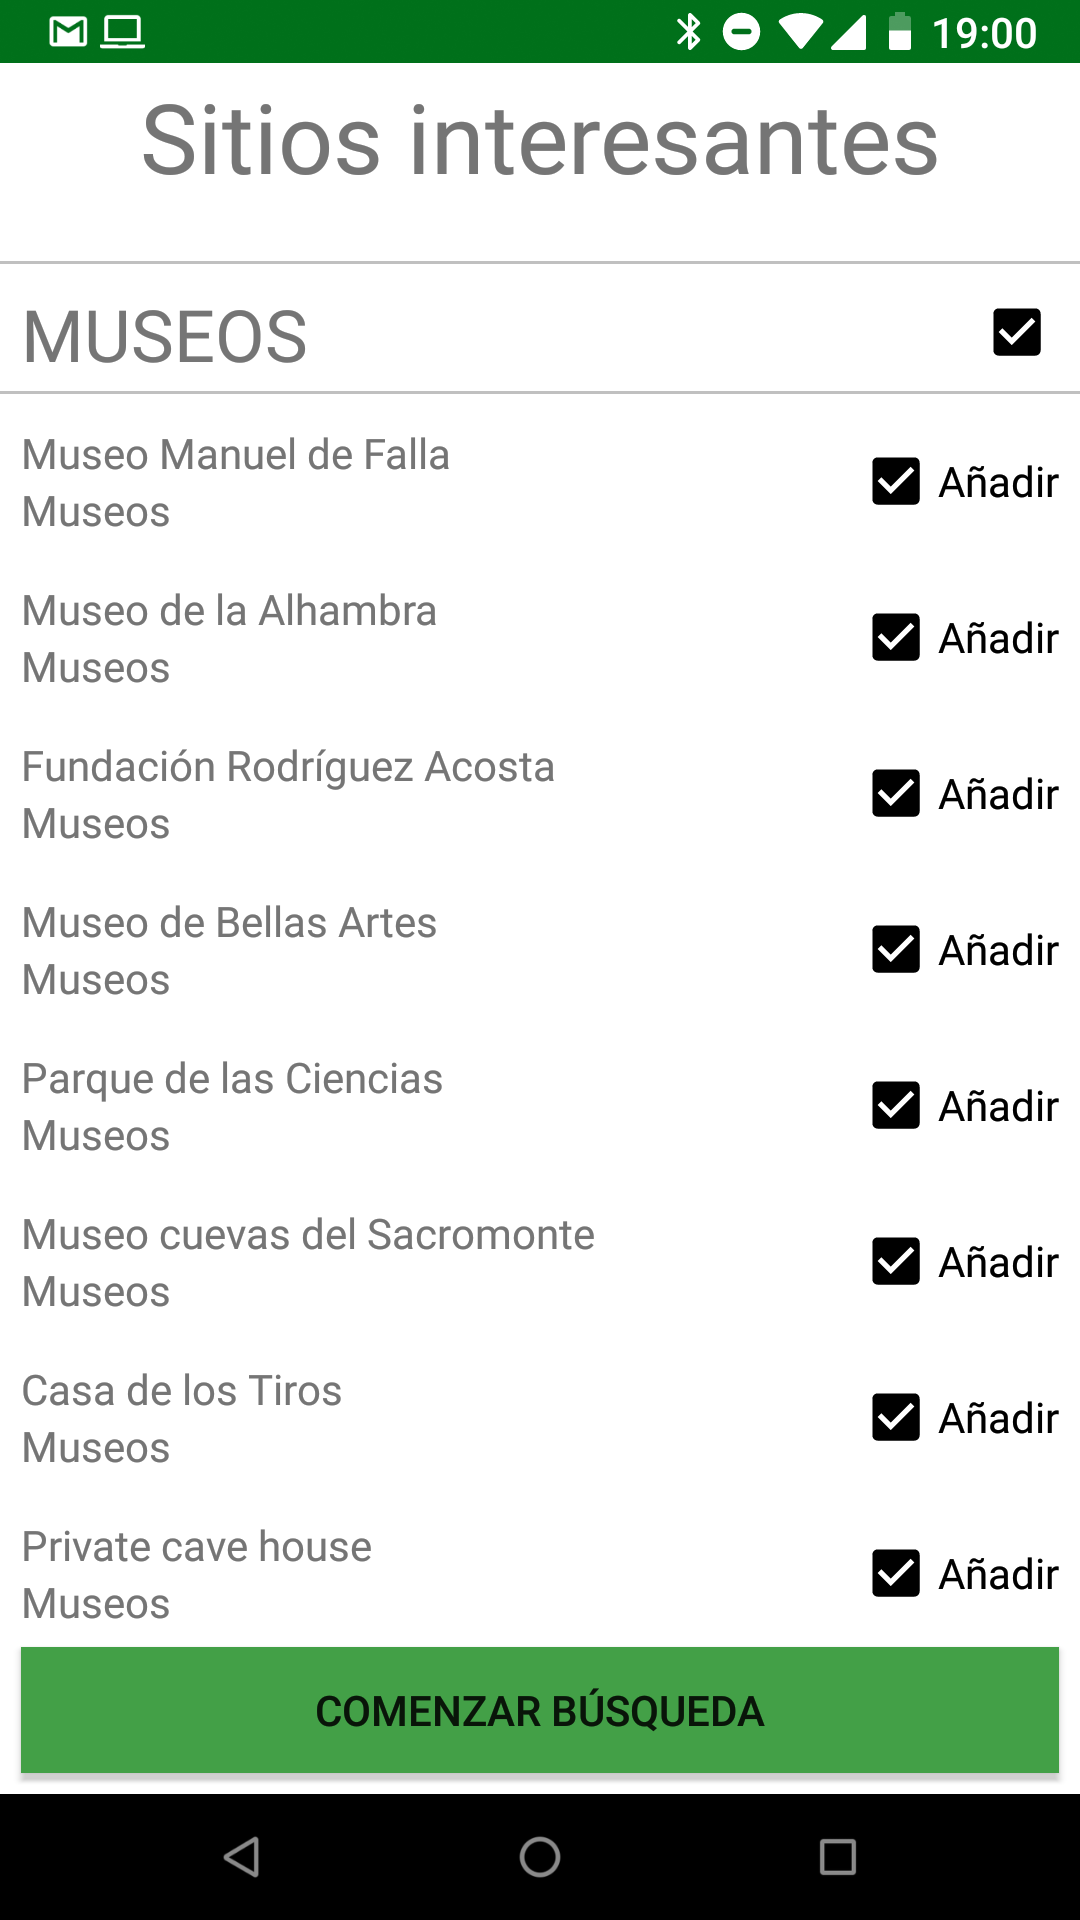
\includegraphics[width=50mm]{imagenes/seleccion_museos}
	\caption{Selección de todos los museos disponibles dentro de la aplicación.}
	\label{fig:selec_museos}
\end{figure}
\begin{figure}[H]
	\centering
	\subfigure{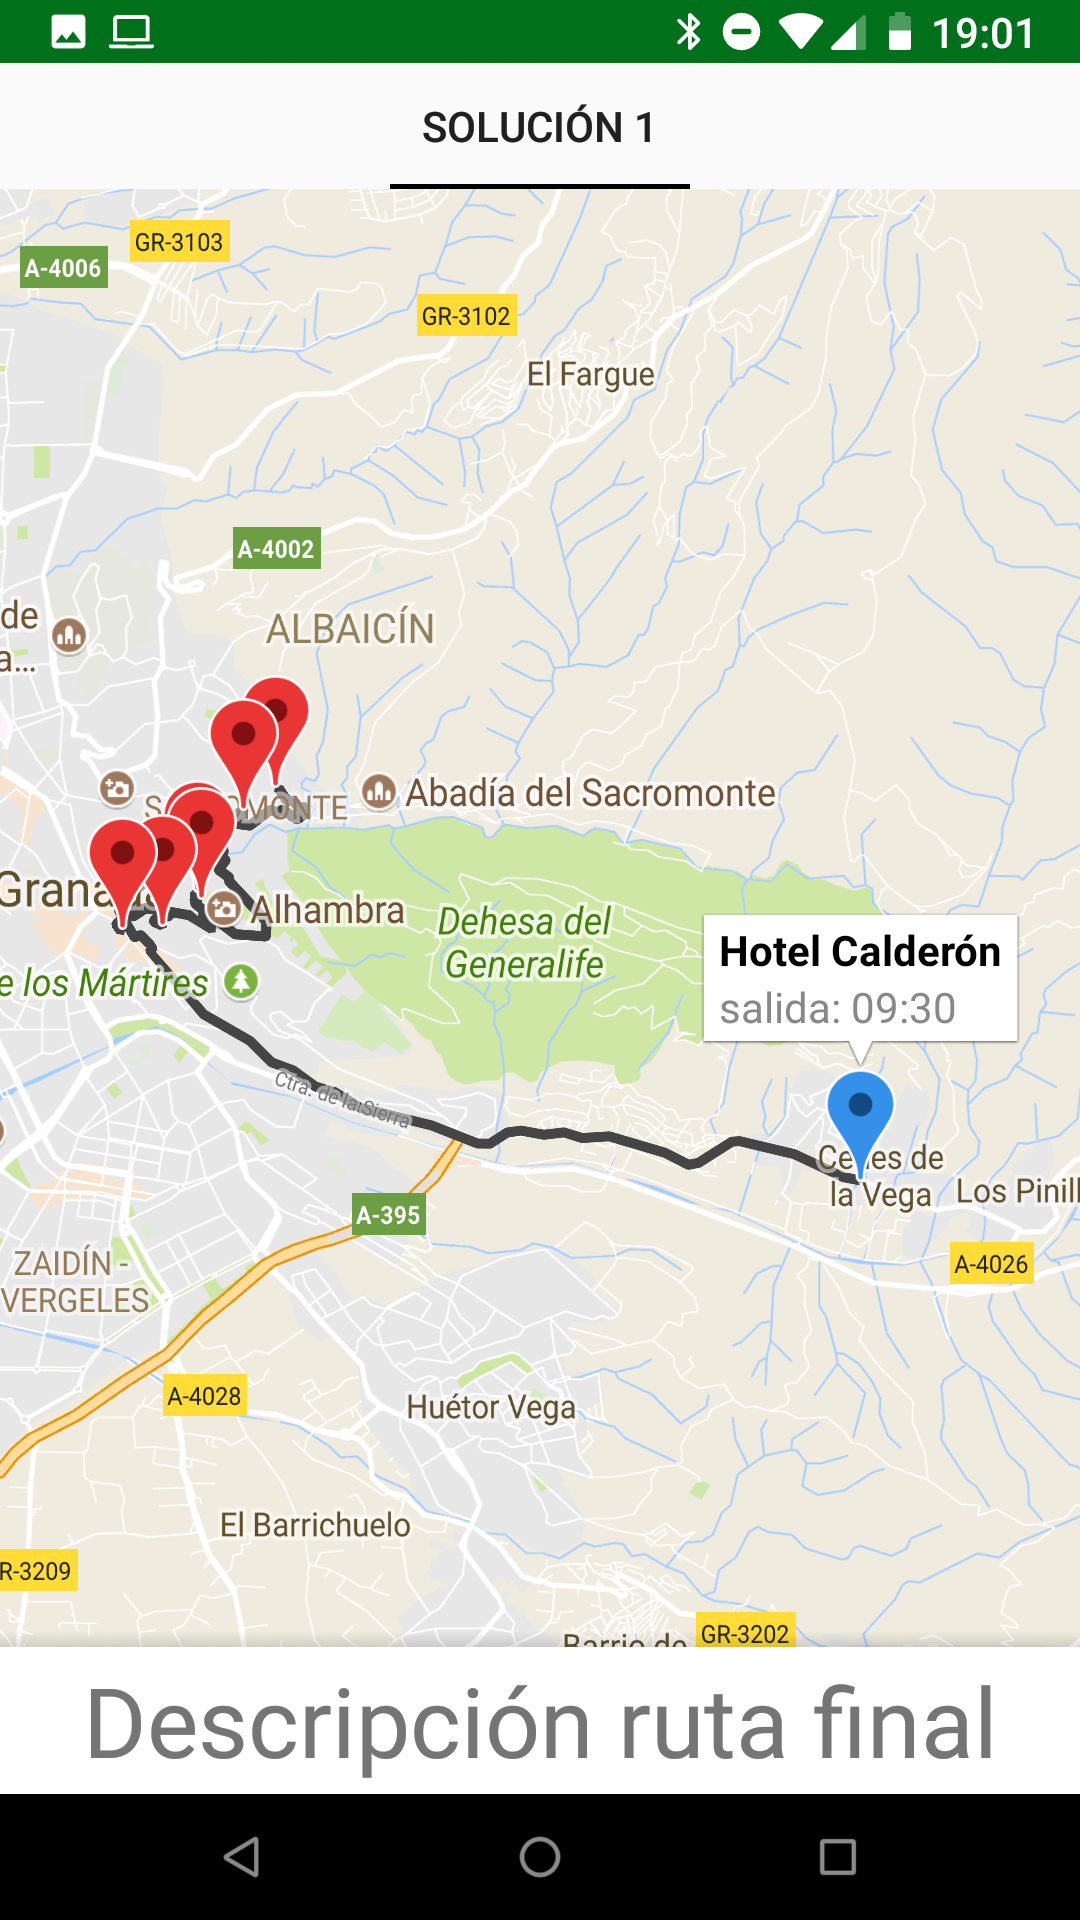
\includegraphics[width=40mm]{imagenes/salida_1}}
	\subfigure{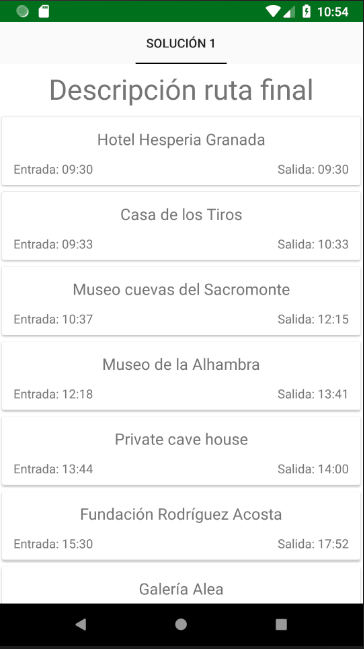
\includegraphics[width=40mm]{imagenes/descripcion_ruta}}
	\caption{Ruta obtenida para el alojamiento seleccionado y todos los museos seleccionados.}
	\label{fig:salida}
\end{figure}

\section[Caso 2]{Ruta sobre un conjunto específico de puntos de interés}
Si se da el caso de que el usuario quiera visitar unos puntos de interés también puede hacerlo; para este ejemplo se van a seleccionar el mirador de San Nicolás, la Hermita de San Miguel Alto, la Catedral de Granada y el Parque de las Ciencias. Para seleccionar dichos puntos, el usuario debe buscarlos dentro de la lista; al igual que se muestran en las figuras \ref{fig:seleccion_multiple}.\newline

Tras esto, el usuario deberá iniciar la búsqueda para pulsar el botón \enquote{Comenzar búsqueda}. Tras esto, se mostrará el resultado, dicho resultado es el que se puede ver en las figuras \ref{fig:salida_2}.Al ser pocos puntos de interés, la solución selecciona todos los puntos de interés.\newline

\begin{figure}[H]
	\centering
	\subfigure{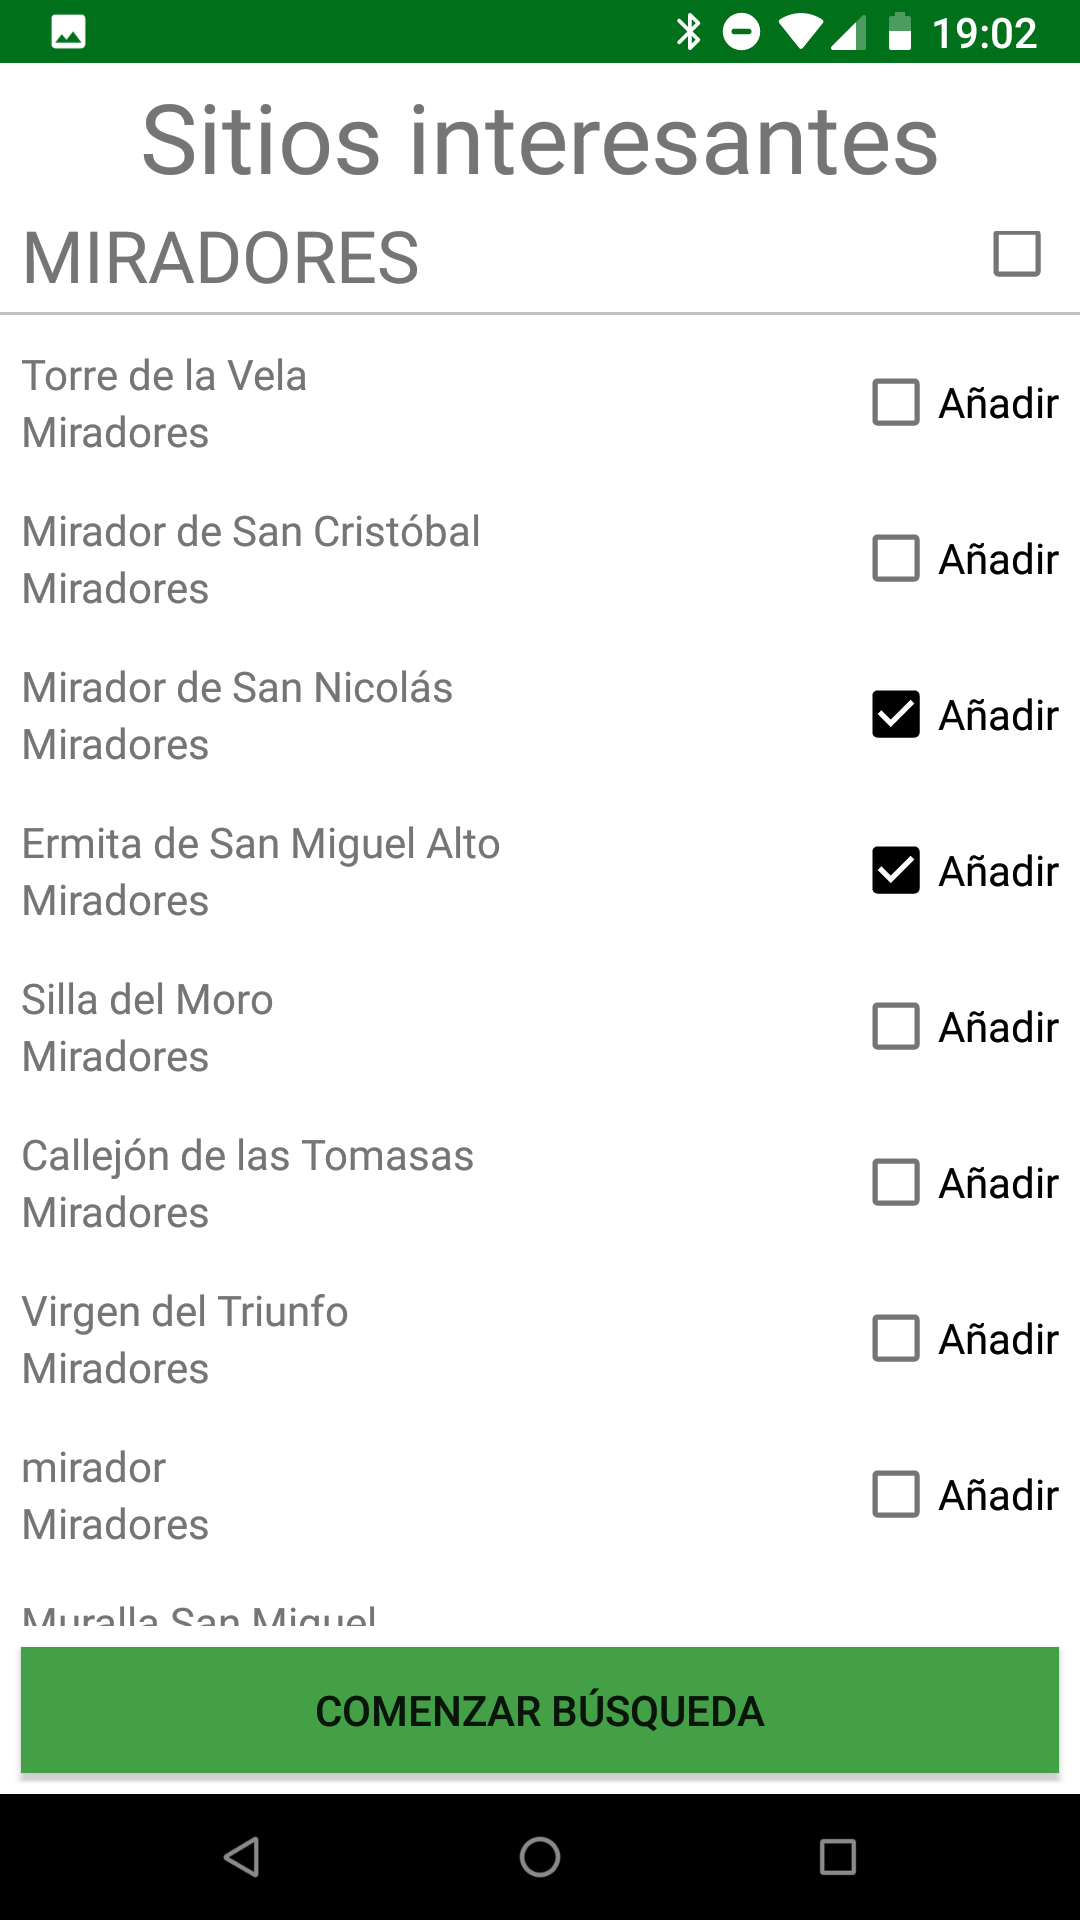
\includegraphics[width=45mm]{imagenes/seleccion_miradores}}
	\subfigure{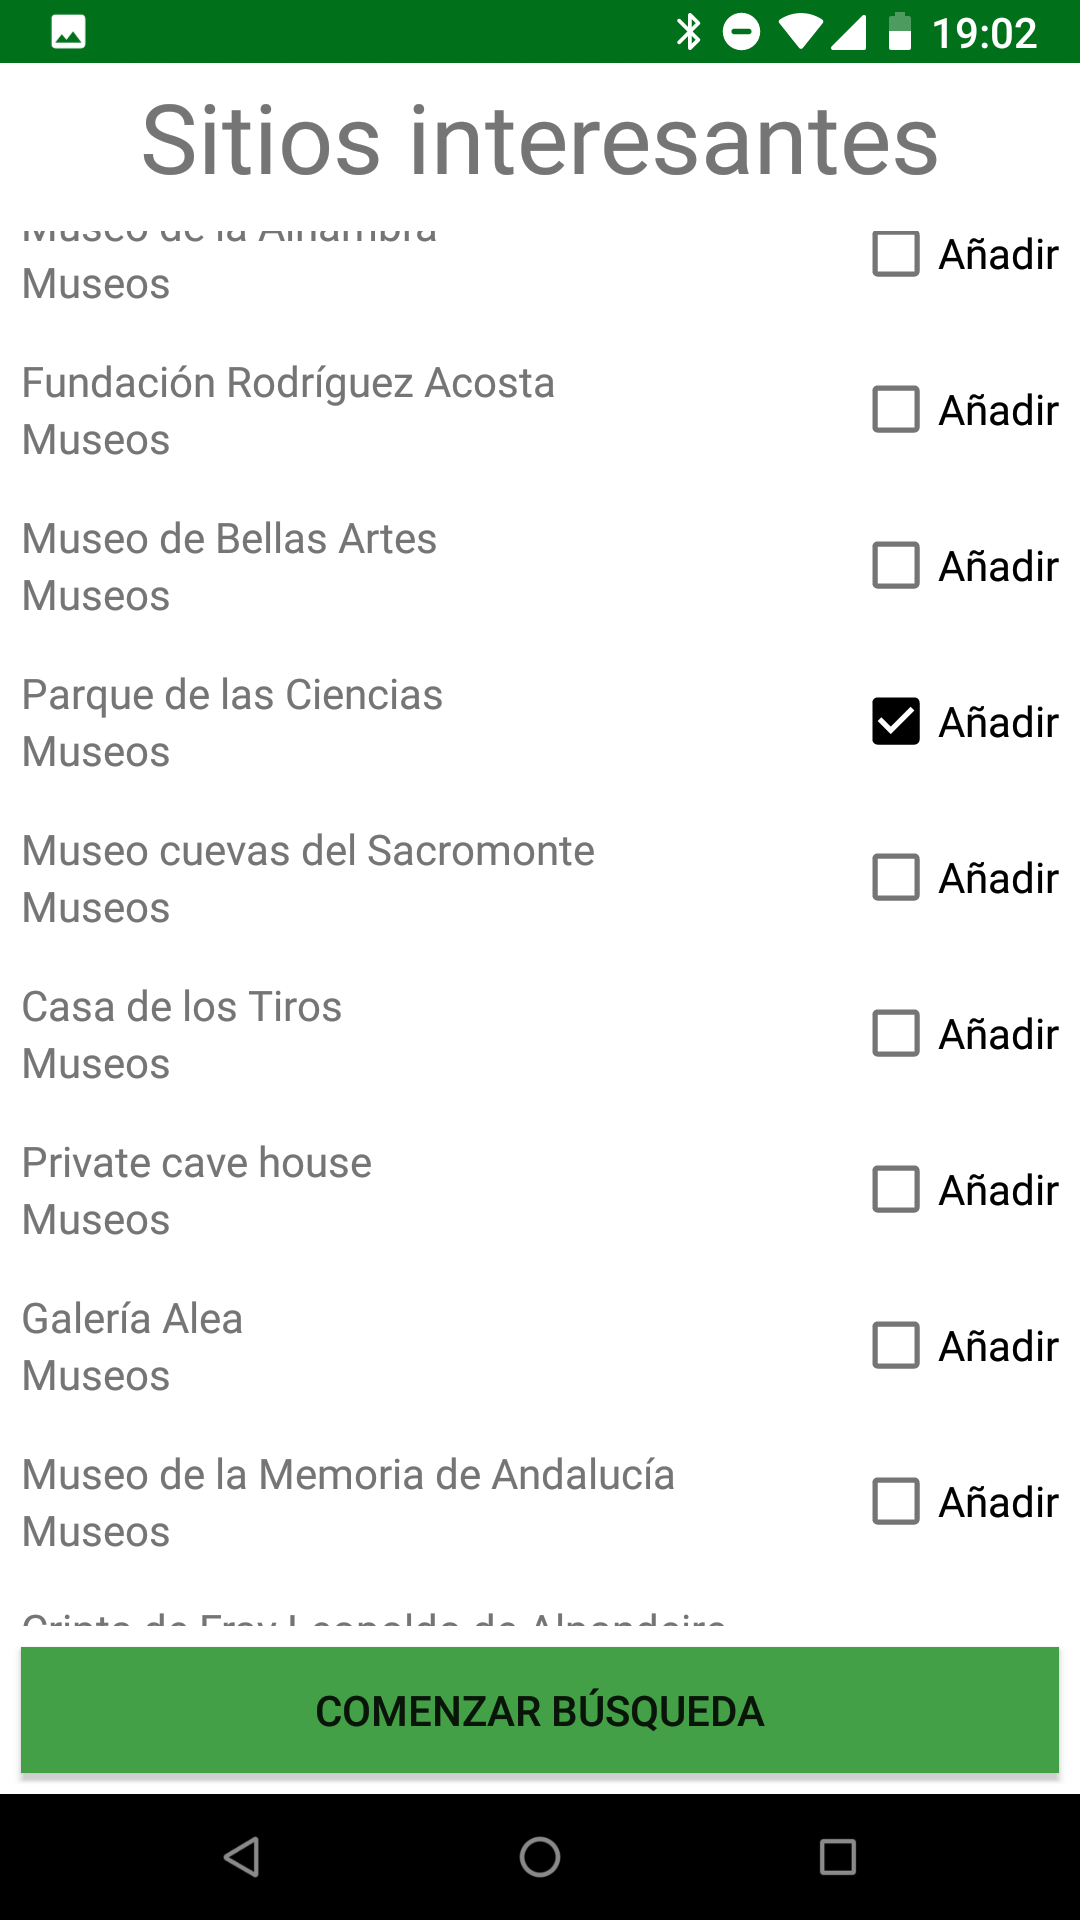
\includegraphics[width=45mm]{imagenes/seleccion_parque}}
	\subfigure{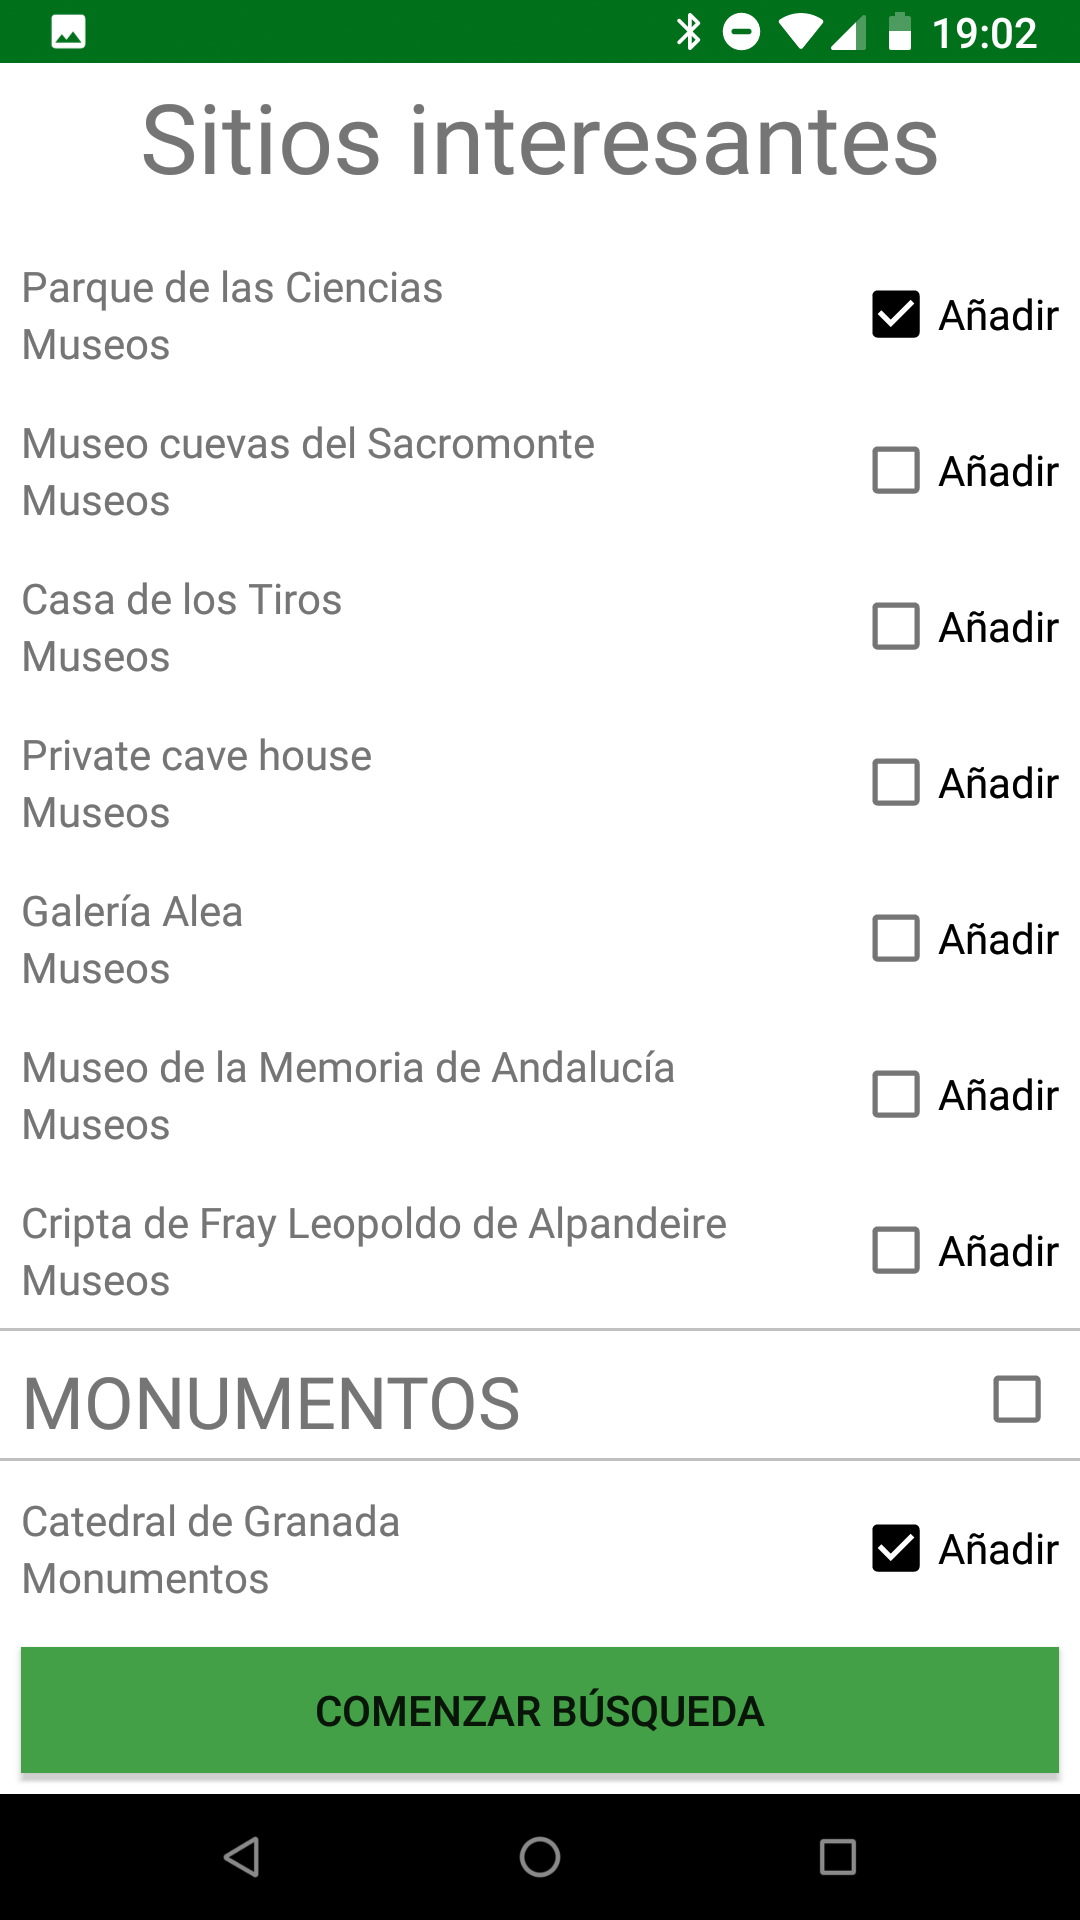
\includegraphics[width=45mm]{imagenes/seleccion_catedral}}
	\caption{Selección de un subconjunto específico de punto de interés.}
	\label{fig:seleccion_multiple}
\end{figure}
\begin{figure}[H]
	\centering
	\subfigure{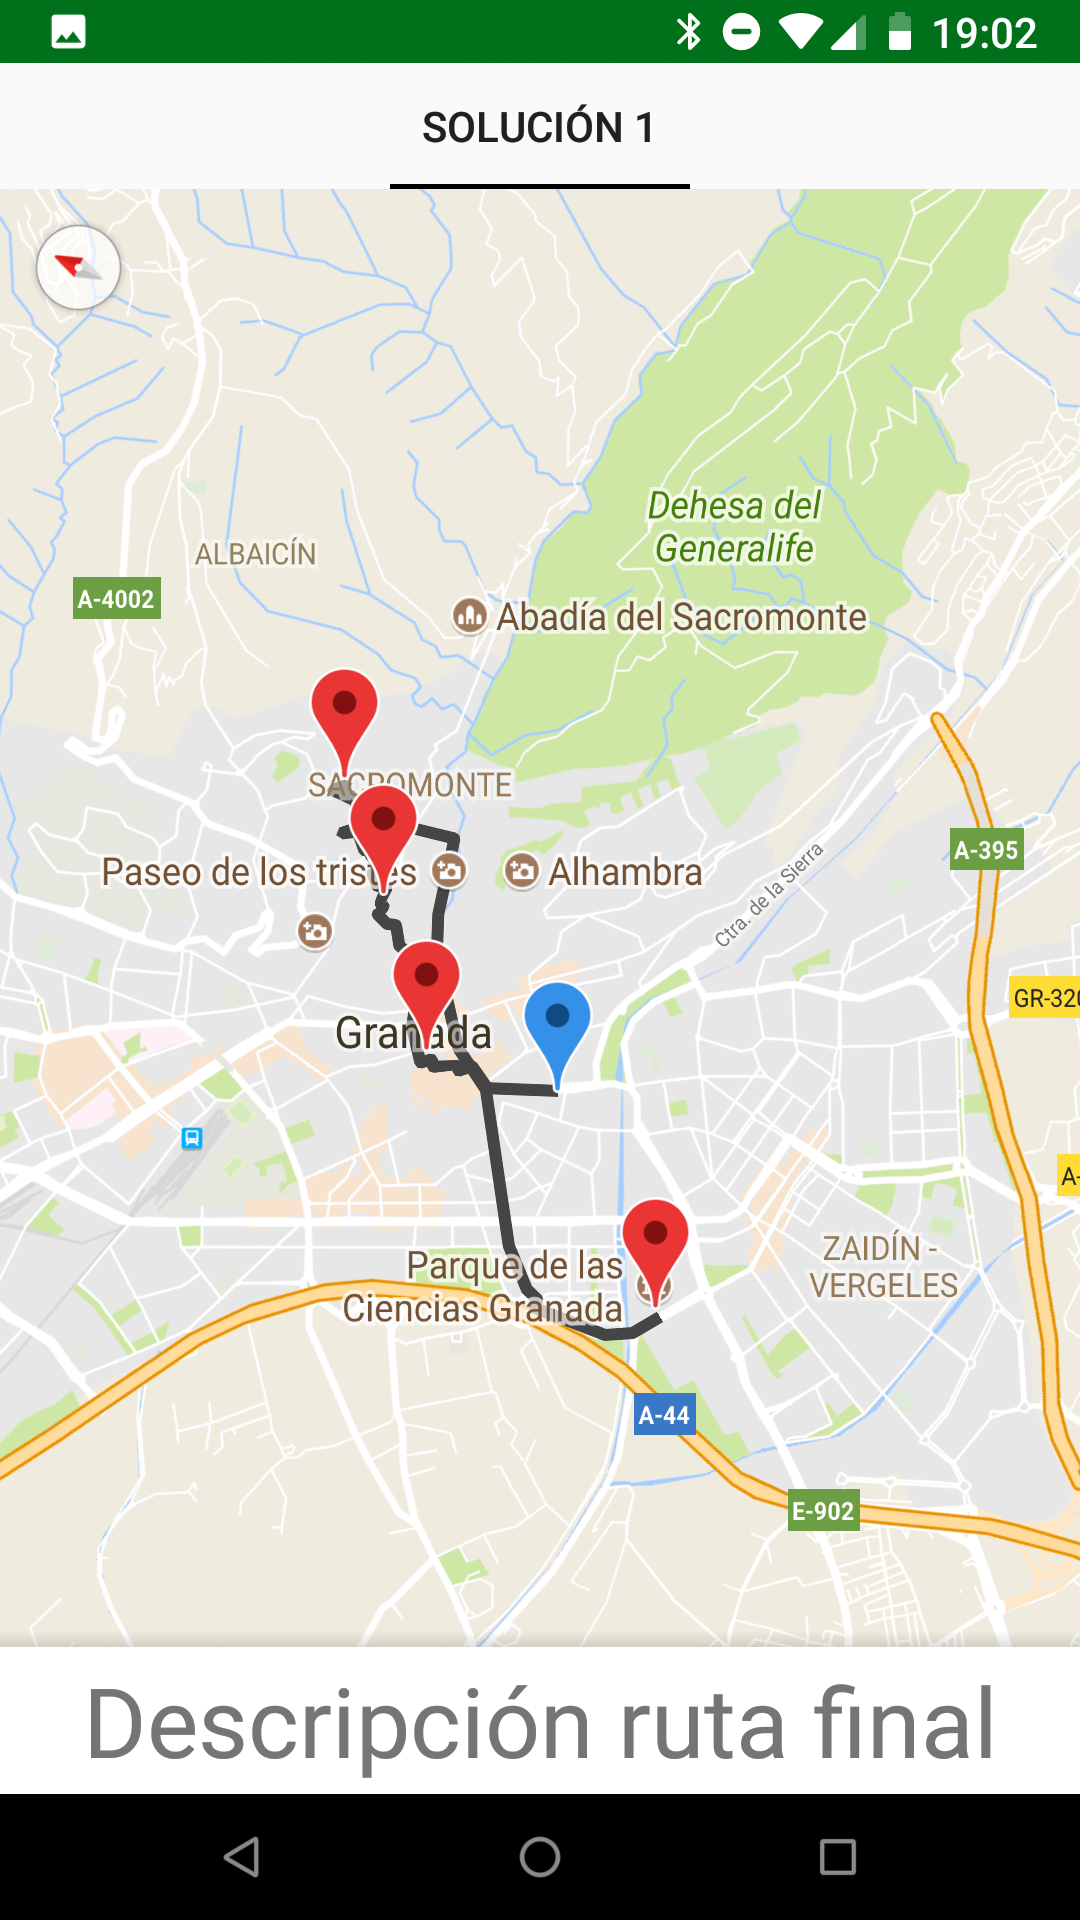
\includegraphics[width=40mm]{imagenes/salida_2}}
	\subfigure{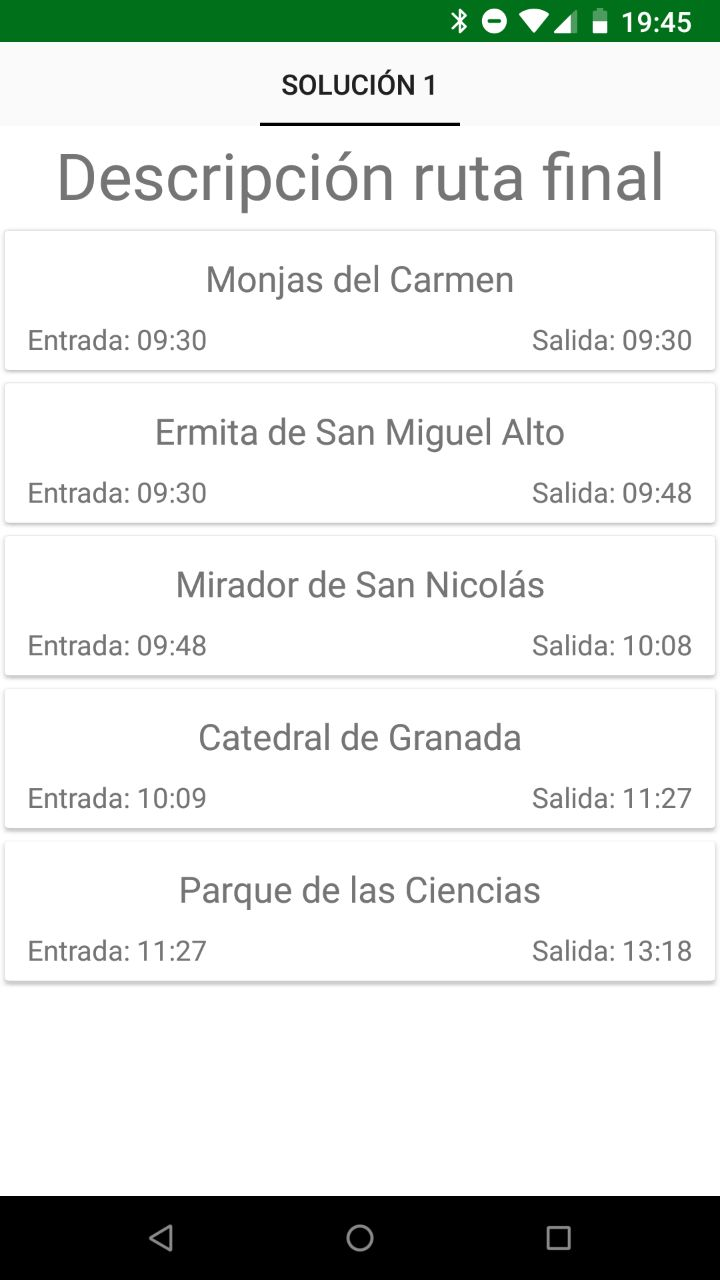
\includegraphics[width=40mm]{imagenes/descripcion_2}}
	\caption{Ruta calculada para el conjunto de puntos de interés.}
	\label{fig:salida_2}
\end{figure}